\section{Problemanalyse}
Gruppen vil indledende for dette projekt undersøge hvordan man gennem tiden har anvendt databehandling til at skjule, eller kryptere, informationer. Målet med denne undersøgelse er et forsøg på at at finde ud af hvorfor de krypteringsmetoder der findes i dag er som de er, og hvorfor de bruges. 
Samt at undersøge, om man ved hjælp af denne forståelse for fortiden, vil kunne danne en metode til at sende beskeder igennem et socialt medie, uden at personer, der ikke besidder kendskab til beskeden, vil vide, at det faktisk er en hemmelig "krypteret" besked.

\newpage

\subsection{Hemmelig kommunikation før internettet}
I dette afsnit vil vi kigge ind i hvordan man tidligere har brugt Kryptografi, altså i tiden inden internettets udbredelse, som skete i det sene 1980. \\
Dog for at skabe klarhed over begrebet kigger vi først på selve definitionen af Kryptografi og hvad dets endelige mening er. 
Kunsten at kryptografere betyder, at skjule information ved at transformere en mening ind i en forudbestemt algoritme.
Dette vil sige at kryptografering ikke bolt betyder at skjule, eller hemmeliggøre en støre mening, men næremere betyder det at transformere noget førhenværende forståeligt, til noget der kun kan forståes, ved brug af en bestemt metode.\cite{MeningOfCryptography}\\
Grundet denne definitionen, kan man også argumentere for, at alle de verdens forskellige sprogs bogstaver og tegn, enten har været, eller stadig er, en form for uforståelig kryptografi, og derfor skal vi kigge på det ældgamle Egypten, 1900 B.C. for at finde de ældste daterede tegn på, eller former for, Kryptografi.\cite{PastCryptography} Selv om man dog også kan diskutere hvorvidt der forefindes noget ældre, så som hulemændenes forskellige væg tegninger.
\begin{figure}[H]
    \centering
    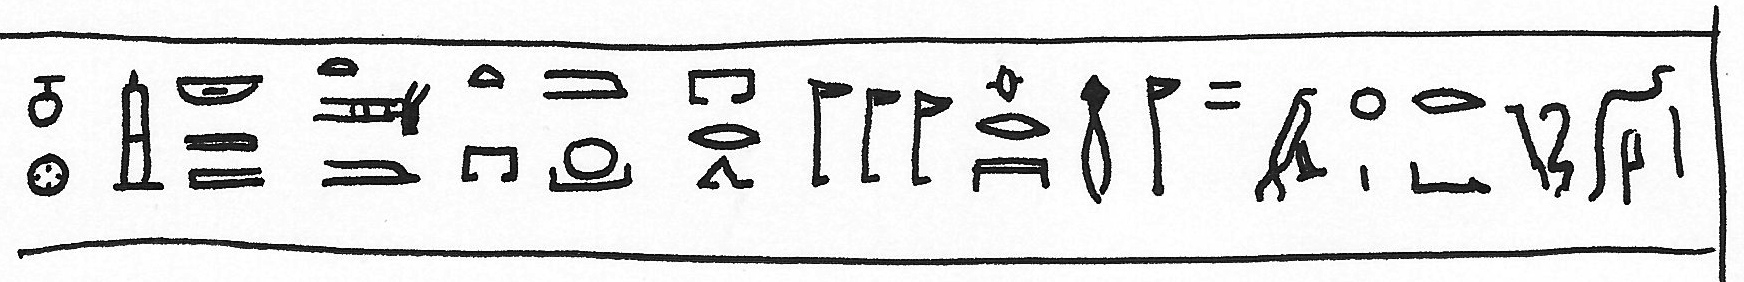
\includegraphics[width=0.8\textwidth, angle =0]{Projectdoc/egypten14.jpg}
    \caption{Egyptiske Hieroglyffer}
    \label{fig:hieroglyffer}
\end{figure}
\noindent
Disse hieroglyffer siges nemlig at være menneskets første form for tekst, og må derfor i begyndelsen ikke have været for alle at forstå. Dog som tiden udviklede sig, lærte det almene Egypten at tolke hieroglyffer, og denne første kryptografi, "De Egyptiske hieroglyffer [Se Figur: \ref{fig:hieroglyffer}]", blev til et anerkendt sprog.
Herefter er de næste former for Kryptografi selvfølgelig alle de andre sprog som efterhånden viste sig, og senere udbredte sig til det almene i de enkelte lande.\\
I takt med denne udbredelse viste der sig dog et nyt behov, behovet for at kunne skjule sine beskeder for andre, der også kunne læse eller skrive ens eget sprog. Den første løsningen på dette behov skal findes i årene omkring 500 B.C.\cite{PastCryptography} \\
\begin{figure}[H]
    \centering
    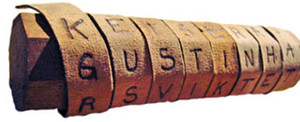
\includegraphics[scale=1.2]{Projectdoc/Problemanalyse/Illustrationer/Scytale.jpg}
    \caption{En Spartansk Scytale}
    \label{fig:scytale}
\end{figure}
\noindent
Da det stadig i denne tid kun var de færreste, der kunne læse og skrive, betød dette at de der faktisk kunne, reelt ikke havde den bedste forståelse for bogstavernes sammenhæng, og Spartanerne kunne derfor opfinde en af de første former for kryptering, "Den Spartanske Scytale [Se Figur:\ref{fig:scytale}]". Denne Spartanske Scytale var en cylinder, hvorom man viklede noget at skrive på, herefter skrev man sin besked på de enkelte sider, og således når man fjernede cylinderen kunne man ikke forstå sammenhængen før man havde en ligeledes størrelsesmæssig cylinder. Denne kryptering ville dog i dag ikke være særlig svær at dekryptere, og kendes også i flere former under bogstavs transponering.\\
Den næste daterede form for kryptering findes allerede små 500 år efter, i det gamle Rom, regeret under Julius Caesar, og siges faktisk også at være opfundet af Julius Caesar ham selv.\cite{PastCryptography}\\ 
Det romerske militær havde brug for at skjule deres strategiske beskeder for fjenden, som ofte fangede de Romerske budbringer, i forsøget på at danne et militærisk modtræk. Ceasar opfandt derfor, den største af de nu tids kendte kryptografi's metoder, kaldet bogstavs substitution eller "A-K Koden".\\
A-K Koden går i alt sin simpelhed ud på, at man flytter alfabetet en vis grad, f.eks. i A-K ville "ABCD" skrives "KLMN", eller i A-S ville "ABCD" skrives "STUV".\cite{TheSecretLanguage}
Som førnævnt er denne bogstavs substitution den mest udbredte og kendte kryptografi's metode, og er derfor også den mest udviklede. A-K Koden findes nemlig også i et utal af andre former.\\ 
F.eks. i formen af "Det hemmelig kodeords A-K", der udføres ved at først vælge et kodeord, "KODEORD", hvorefter kodeordets bogstaver flyttes til starten af alfabetet for tilsidst af fortsættes resten af alfabetet, derfor ville "ABCDEFGHIJKLMNO" skrives "KODEORDABCFGHIJ", således at "HEJ" ville skrives "AOC". \cite{TheSecretLanguage}
Andre former af A-K Koden kunne være "Alberti-Vigeneres Cipher" opfundet i midt 1400 tallet, "The Vingenere Cipher" fra 1500'erne, eller Jefferson's Wheel Cipher fra det sene 1700,\cite{PastCryptography} der alle som Caesar's koncept, fungere ved udbytning af bokstavernes rækkefølge, men dog i de nævnte også ved hjælp af et værktøj, som ved Den Spartanske Scytale.



--------------- NOTER --------------\\
Som to nyere kan nævnes WWII's kryptografi maskiner, Morsing, og
Allernyest The Da Pinchi Code, (Tyvene idag bruger denne kode.) the hobo code
\newpage
\subsection{Internettets oprindelse}
I dag anvendes internettet i næsten alle hjem og er udbredt i alle lande. Derfor vil der i dette afsnit blive undersøgt hvad internettets oprindelige formål egentligt var, og om denne idé måske vil kunne anvendes med hensigt til projektets formål. 
\\\\
\noindent 
Internettet, som er det fysiske netværk, liggende imellem enheder, ansvarligt for leverance af data, havde sin spæde start i 1962 da J.C.R. Licklider beskrev hans "Galactic Network" koncept. Hvad han beskrev var essentielt det der i dag kendes som internettet. Han forestillede sig nemlig et netværk hvorpå enhver forbunden computer kunne tilgå data og programmer på ethvert givet site. Allerede i 1967 blev planen for ARPANET publiceret, og kun to år senere blev de første to nodes koblet på ARPANET (nodes her værende forstået som netværksudstyr og ikke endpoints).\\ 
I den efterfølgende måned blev den første host to host besked sendt. Dette var første gang data blev flyttet fra en computer til en anden, uden udveksling af et fysisk medium. Den første offentlige demonstration af ARPANET foregik i 1972, hvilket også var samme år hvor den første elektroniske mail applikation blev lavet. 
Disse to ting viste hermed muligheden for en helt ny anvendelse af computere.\cite{brief_history_of_the_internet}
\\\noindent
Udviklingen stoppede ikke her, da en sammenkobling af flere ARPANET lignende netværk blev forslået kun to år senere. Denne sammenkobling af netværk gav anledning til udtrykket "internetværk". Dette forslag endte ud i skabelsen af TCP/IP standarden som muligjorde den videre udvidelse af hvad der blev til internettet.\cite{The_development_of_the_internet}

\subsubsection{Hvorfor blev internettet lavet?}
Behovet for et computer baseret kommunikationsnetværk opstod omkring højden af den kolde krig. På denne tid blev der overvejet mange mulige implikationer af, hvad der syntes som en uundgåelig, atomkrig. Én af disse overvejelser gik på hvordan man kunne kommunikere over lange afstande, i tilfælde af at telefonnettet blev ødelagt. Hvad der var brug for, var et system som kunne fungere selvom enkeltstående komponenter blev beskadiget. Det var i denne forbindelse at "Galactic Network" konceptet opstod.\cite{The_Invention_of_the_Internet}
\\\noindent
Projektet startede derved under det amerikanske forsvars ministerium, og var derfor af militær karakter i starten. Dette begyndte at ændres da ARPANET blev forbundet til stadig flere steder, mange af disse værende universiteter. Denne løbende udvidelse af ARPANET gav anledning til, at projektet nu blev videre udviklet af såvel staten, som private. Selvom det startede med et behov for pålidelig kommunikation i en krise, endte ARPANET derfor med at være værdifuldt blot i effektiviteten af kommunikationen som det tilbød, og den data som den indeholdt.

\newpage
\newpage
\subsection{Statslig censur af internettet}
Den global internet frihed er på syvende år i træk stadig dalende \cite{FreedomHouseRapport2017}, lyder det fra den uafhængige frihedskæmpende organisation Freedom House i deres årlige rapport "Freedom on the Net". Freedom House har til formål at fremme frihed og demokrati rundt omkring i verden, blandt andet ved at fortage dybdegående analyser og ved at fortale menneskerettigheder \cite{FreedomHouseAbout}. Den årlige "Freedom on the Net" rapport afdækkede i de to nyeste udgivelser (2016 og 2017) internetfriheden for mindst 87\% af verdens internet benyttede befolkning og giver hvert år en resumering af hvilke trends der havde størst betydning for deres samlede konklusion. 

Hvert af de 65 lande der årligt bliver afdækket, får tildelt sig en numerisk score alt efter hvor god eller ringe deres internet frihed har været. Denne score går fra 0 til 100 og er ydermere opdelt i 3 overordnet kategorier: Free (0 - 30 points), Partly Free (31 - 60) og Not Free (61 - 100). En score er også bestemt ud fra 3 overordnet kategorier: Forhindringer for adgangen til nettet (Giver 0 - 25 points), restriktioner på indholdet (0 - 35) og overtrædelser af brugernes rettigheder (0 - 40) \cite{FreedomHouseRapportMethodology}.

\subsubsection{Censur af kommunikationskanaler}
I 2016 udgivelsen af rapporten blev den stigende magtmisbrug af de sociale medier samt andre kommunikationskanaler belyst. I 2015 fandt Freedom House frem til at 15 regeringer ud af de 65 undersøgte havde begrænset befolkningens adgang til diverse sociale medier, i 2016 havde dette tal stiget til 24. Brasilien og Tyrkiet endte 2016's undersøgelse med at blive to af de mest bemærkelsesværdige lande, der begge gik et betydeligt skidt tilbage på deres respektive frihedsskalaer, netop på grund af deres magtanvendelse overfor diverse kommunikationskanaler. Brasilien gik fra kategorien "Free" til "Partly Free" da brasilianske domstole indførte en midlertidig blokering af opkald- og tekstkommunikations tjenesten WhatsApp, da WhatsApp nægtede at udlevere brugerdata til bevismateriale. Tyrkiet gik fra kategorien "Partly Free" til "Not Free" efter masseblokeringer af diverse kommunikationskanaler og efterfølgende forfølgelse af borgere der kritiserede Tyrkiets regering. 

Den mest hyppige årsag til regeringers, især autoritære regimers, restriktioner af diverse kommunikationskanaler er for at holde deres befolkninger i skak. Disse restriktioner sker blandt andet når en regering kritiseres, når der mistænkes korruption eller under anden aktivisme. Da disse kommunikationskanaler er så gode til at for samlet folk og organisere protester og lignede, vil visse regeringer bruge deres magt på undertrykkelse. Det er dog ikke kun aktivisme nogle af disse autoritære regimer undertrykker, også homoseksuelle fællesskab, satire, religiøse og modstående politiske overbevisninger bliver undertrykt \cite{FreedomHouseRapport2016}.

\subsubsection{Angreb mod kryptering}
Moderne efterforskning inkludere i højere grad de forskellige kommunikationskanaler når kriminalitet og terroristisk aktivitet skal bekæmpes. Smartphone, computere og online services er i vor tid tætpakket med avanceret kryptering, både for at beskytte virksomhedens brugere men også virksomheden selv. Denne kryptering så myndighederne i blandt andet Kina, Ungarn, Rusland, Thailand, Storbritannien og Vietnam gerne gradbøjet, som led i individuelle lov ændringer indefor området. Disse love kan kræve at virksomheder udlevere backdoor krypteringsnøgler til myndighedernes efterretningstjenester. Dette kan udgøre en kolossal risiko for alle brugerene af det pågældende medie, især de brugere der har brug for en sikker kanal til journalistisk eller aktivisme. Back

VPN'er og Backdoors
\cite{FreedomHouseRapport2017}

\newpage
%\subsection{Den etiske diskussion}
% I det foregående afsnit blev nogle typer og grader af statslig censur gennemgået. I dette afsnit vil der fokuseres på nogle etiske overvejelser, i forbindelse med forskellige landes forsøg på at øge lokal sikkerhed. \\\\
\noindent
% I den vestlige verden er man i højgrad vant til at leve i et samfund, som værdsætter ytringsfrihed og almentgældende menneskerettigheder. På basis af dette har det også været muligt at danne regeringer, som også holder disse værdier højt. På trods af dette har vestlige lande i forskellige grader valgt, at gå på kompromis med basale elementer af privatlivets fred, til fordel for øget sikkerhed mod terrortrusler. Disse er blandt andre videoovervågning i mange vestlige byer, og overvågning af almen internettrafik. Ydermere er efterretningstjenester i stand til at købe information om almindelige personer fra sociale medier såsom Facebook. Den ønskede effekt af disse kompromiser er, at give politi og efterretningstjenester muligheden for, at forhindre terror angreb. Selvom dette lyder ganske fornuftigt, så findes der eksempler på situationer, hvor dette kompromis ikke er helt så simpelt.\\\\
\noindent
% Et godt eksempel på dette er de sager hvor FBI har bedt Apple om, at bryde sikkerheden på et af deres egne produkter\cite{FBI/Apple_encryption}. Naivt ville man måske sammenligne dette med at bede en låsesmed om, at åbne en låst dør. Dette er naturligvis inden for hvad politiet forventer at kunne bede om. Problemet er, at analogien i dette tilfælde ikke holder. Det gør den ikke, da man for at bryde cybersikkerhed bliver nød til at skrive noget software, til at kompromittere en bestemt type enhed. Dette stykke software ville så kunne bruges på alle lignende enheder, eller nemt modificeres til dette, og dette er netop problemet. Hvis blot man kunne være sikker på, at denne software aldrig nogen sinde ville blive misbrugt, så ville det principielt være en funktionel løsning. Men det kan man ikke. I kontrast til en fysisk masterkey, hvor fysiske kopier tager tid, penge og ekspertise at producere, så kan en software baseret masterkey kopieres i det uendelige. På den måde går en umiddelbart fornuftig forespørgsel hurtigt over til at have potentielt store og vidt rækkende konsekvenser.\\\\
\noindent
%Selv hvis det er muligt at udtænke en fysisk masterkey til brydning af cybersikkerhed, ville man stadigvæk være tvunget til, at stole på den regering som har adgang til den. Dette bringer diskussionen videre til forskelle på demokratiske og diktatoriske lande, såvel som dem i gråzonen. Groft sagt stoler man i den demokratiske verden på, at ens basale menneskerettigheder bliver overholdt, ved hjælp af magtens tredeling. Dette burde sikre, at regeringen ikke agerer uden for lovens rammer. Den almene borger stoler derved på, at denne tredeling holder øje med hinanden, og igennem dette sikrer individets rettigheder. Såfremt dette er tilfældet vil regeringen ikke kunne misbruge de værktøjer, som lovgivningen tillader dem at have, fordi domstolene opererer uafhængigt af regeringen, og sørger for, at de overholder lovgivningen. Samtidigt vil domstolene også sørge for, at der ikke bliver vedtaget nye love, som bryder med samfundets mest fundamentale retningslinjer, altså det enkelte lands grundlov. Men når der arbejdes med cybersikkerhed, er de enkelte lande bare ikke isoleret på samme måde, som de har været tidligere. Med dette menes, at selvom ét lands lovgivning tillader deres regering at være i besiddelse af en masterkey, og måske endda at lovligt tvinge firmaer til at lave masterkeys, så betyder dette ene lands beslutning dermed, at sådan en masterkey vil findes, og dermed også at andre regeringer, eller kriminelle, også kunne få anskaffet samme type udstyr, værende fysisk eller digitalt. Dog skal det siges, at så længe regeringer prøver at tvinge firmaer til at lave masterkeys, så har firmaerne mulighed for at gå til en domstol, hvis de mener det ikke er berettiget. Derfor er det vigtigt at overveje de mulige konsekvenser, ikke blot af kriminelle, men også af hele regeringer, som ikke overholder almene menneskerettigheder.\\
\noindent
%I værste fald kunne sådanne forsøg på at øge individets sikkerhed, med hensyn til almen kriminalitet og terror, ende med at yderligere begrænse friheden for store dele af verden, og endda øge cyberkriminalitet markant.


%Tilføre afsnit om... ?

\newpage